\section{Método de obtención de tiempos y gráficas}
	\begin{enumerate}
		\item El programa preguntará por el tamaño del problema (la longitud del array)
		\item También podemos elegir el mayor entero a generar (un entero puede tener un valor 				máximo de $2147483647$ )
		\item El programa preguntará por el salto \emph{(gap)} entre iteraciones.  Cuanto menor 					sea el tamaño de la iteración, más ajustada será la gráfica.  Para asegurarnos que 					recorremos hasta el último elemento del array el salto debe ser múltiplo de $5$.
		\item En primera instancia se genera un array con números aleatorios que sirve como base 					para las ordenaciones.  De esta manera las copias del array original se hacen del 					tamaño que corresponde a la iteración.  Así, si el tamaño del array a ordenar en cada iteración es de $n$ 					elementos, el programa copia el array en intervalos de $gap$ elementos hasta alcanzar el tamaño máximo del problema $(n)$.
		\item El programa genera un archivo con los datos separados por un salto de línea.  Cada 					línea contiene el tamaño del problema y el tiempo empleado para la ordenación expresado 			en segundos.
		\item Con los archivo de datos, puede ejecutarse el script de órdenes con la sintaxis de 				\textbf{gnuplot} para crear los arhivos de imagen con las gráficas de las métricas 					generadas.
	\end{enumerate}


\section{Análisis de resultados}
\begin{itemize}
\item Tamaño del problema: $100000$\footnote{Todos los resultados han sido generados en un ordenador Apple Imac, Mac Os X 10.8.2, Procesador Intel Core i5 a 2,5Ghz (4 núcleos), 4 Gb de RAM a 1333 Mhz DDR3.}
\item Máximo entero generado: $125000$
\item Salto entre iteraciones: $100$
\end{itemize}
\newpage
%Gráfica de ordenación por inserción
\subsection{Ordenación por inserción \cite{CORMEN}}
Su complejidad es de $O(n^2)$. Un buen algoritmo de ordenación para un número pequeño elementos. Funciona de la manera análoga a la que se ordenaría un mazo de cartas:
\begin{enumerate}
	\item Empezamos con la mano izquierda vacía y las cartas boca abajo sobre la mesa.
	\item A continuación, cogemos una carta de la mesa, y la insertamos en la posición correcta 			en la mano izquierda.
	\item Para encontrar la posición correcta en la que insertar la carta, se compara con cada 			una de las cartas que ya tenemos en la mano izquierda, recorriendo de derecha a 					izquierda.
\item En todo momento, las cartas sujetas con la mano izquierda se ordenan, permaneciendo las 			cartas originales sin ordenar encima de la pila en la mesa.
\end{enumerate}

	\begin{figure}[H]
  		\centering
   		 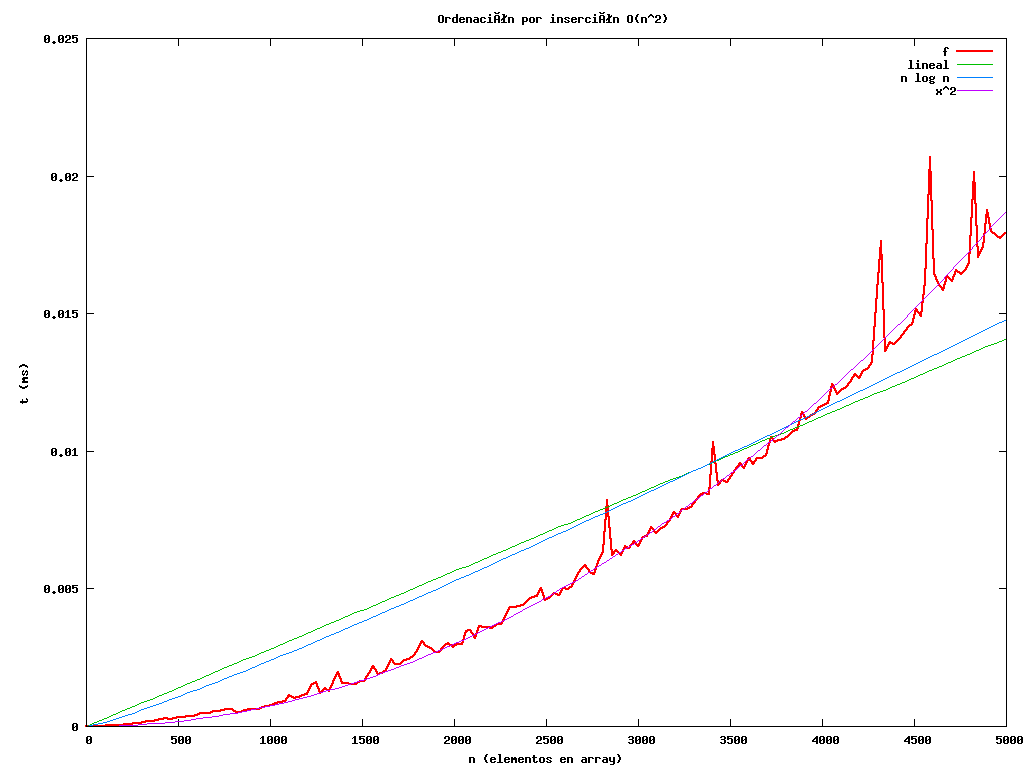
\includegraphics[width=1.0\textwidth]{insertion-sort.png}
  		\caption{Ordenación por inserción}
 			 \label{fig:insertion}
		\end{figure}

\newpage
%Gráfica de ordenación por selección
\subsection{Ordenación por selecci\'on}
Es un algoritmo de ordenación por comparación. Su complejidad es de $O(n^2)$. Resulta ineficiente en tamaños de problema grandes, y suele funcionar peor que la ordenación por inserción. Se caracteriza por su sencillez, y también tiene ventajas de rendimiento sobre algoritmos más complicados en determinadas situaciones, sobre todo cuando la memoria auxiliar es limitada.\\
El algoritmo divide la lista de entrada en dos partes: la lista secundaria de los elementos que ya están ordenados, dispuestos de izquierda a derecha, y la lista secundaria de los elementos restantes a ser ordenados, ocupando el resto de la lista. Inicialmente, la sublista ordenada está vacía y la sublista sin ordenar es la lista original menos los elementos ordenados. El algoritmo continúa encontrando siempre el elemento inmediatamente superior (según orden de clasificación) y lo cambia con el último elemento del array.

	\begin{figure}[H]
	  \centering
	    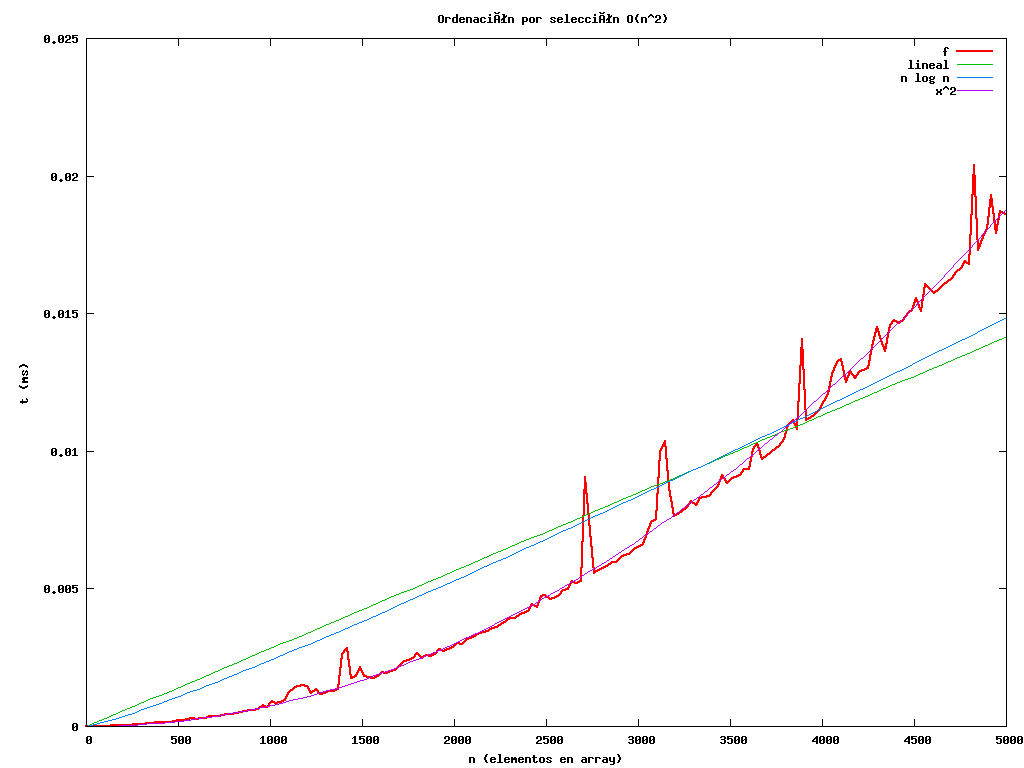
\includegraphics[width=1.0\textwidth]{selection-sort.png}
	  \caption{Ordenación por selección}
	  \label{fig:selection}
	\end{figure}

\newpage
%Gráfica de ordenación por burbuja
\subsection{Ordenación por burbuja}
Es un algoritmo por comparación.  Recorremos los elementos del array de derecha a izquierda, comparando cada elemento con el siguiente e intercambiándolos en caso de estar desordenados.
\subsubsection{Rendimiento}
Para ordenar un vector de $n$ elementos, el algoritmo siempre realiza el mismo número de comparaciones:
\[n\]
	\begin{figure}[H]
	  \centering
	    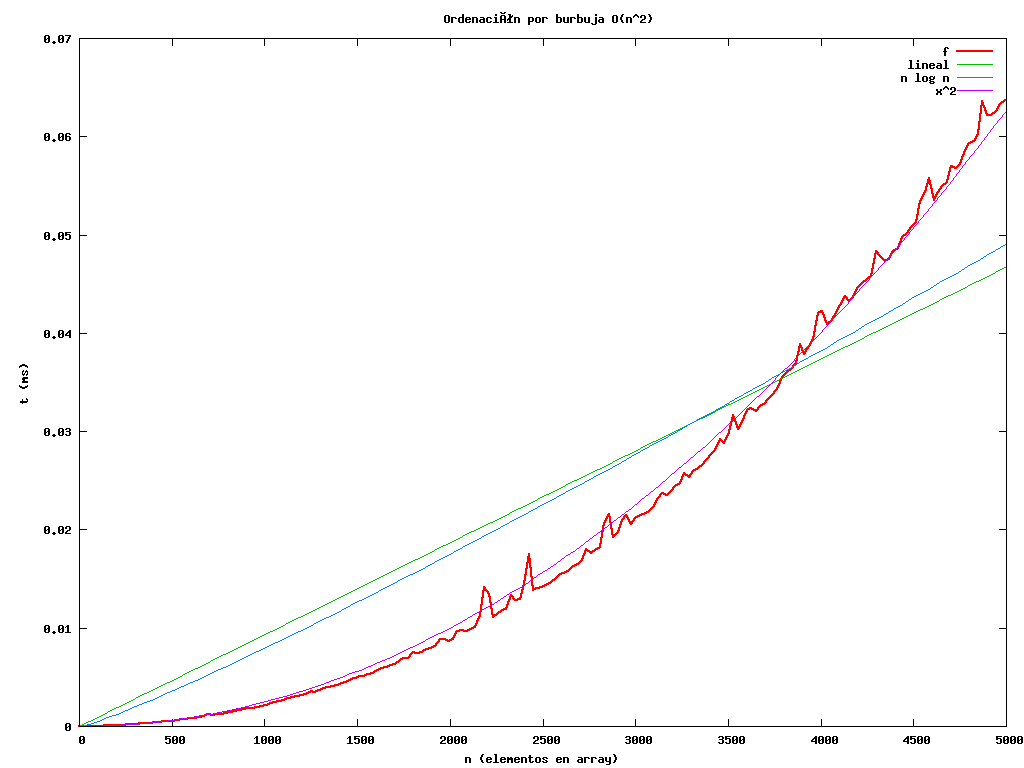
\includegraphics[width=1.0\textwidth]{bubble-sort.png}
	  \caption{Ordenación por burbuja}
	  \label{fig:bubble}
	\end{figure}

%Gráfica de ordenación rápida
\subsection{Ordenación r\'apida}

	\begin{figure}[H]
  		\centering
   	 	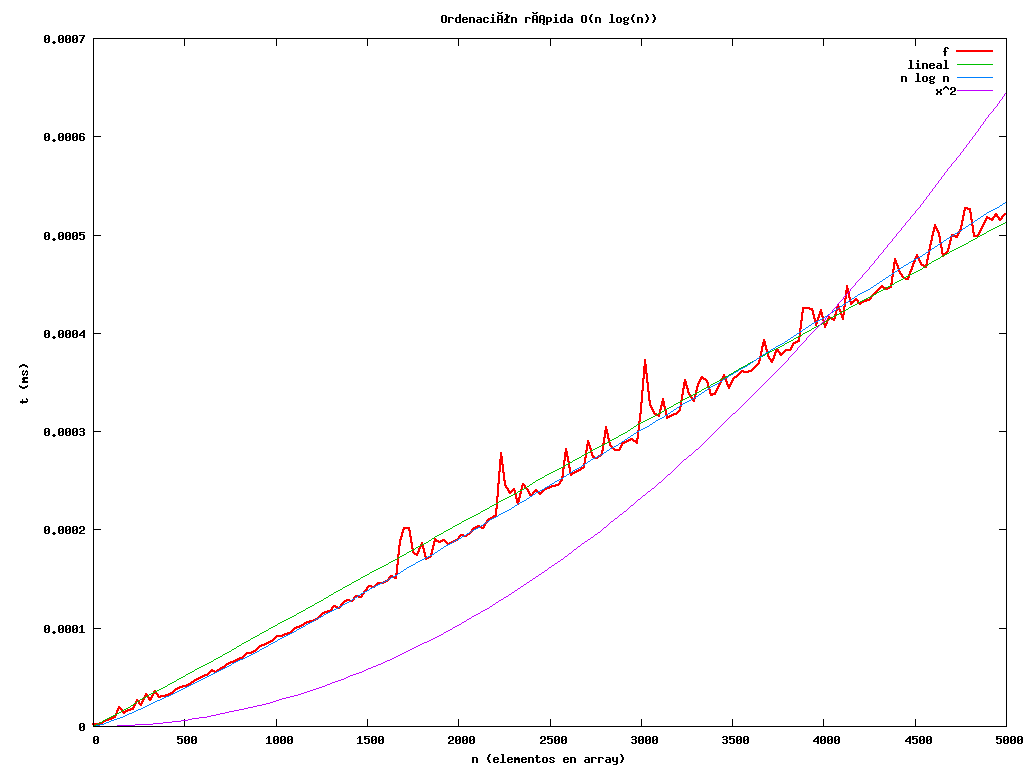
\includegraphics[width=1.0\textwidth]{quick-sort.png}
  		\caption{Ordenación rápida}
  		\label{fig:quick}
	\end{figure}
	
\subsection{Ordenación por mezcla}

	\begin{figure}[H]
  		\centering
   	 	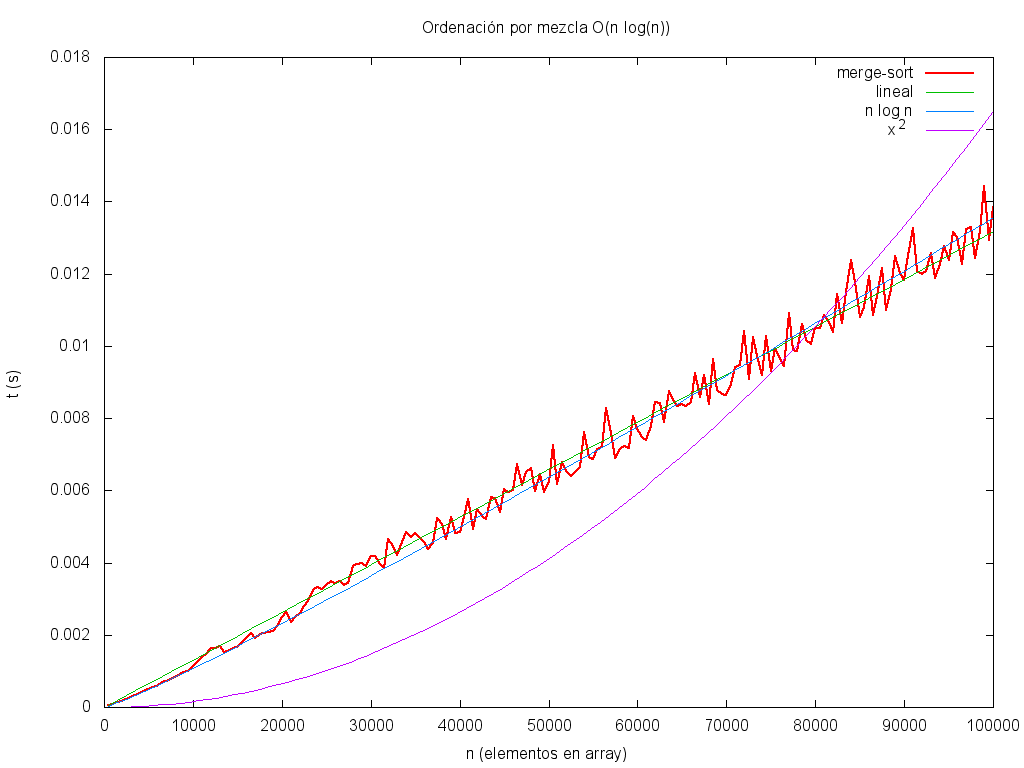
\includegraphics[width=1.0\textwidth]{merge-sort.png}
  		\caption{Ordenación por mezcla}
  		\label{fig:merge}
	\end{figure}
